% Auto-generated by scripts/failure_modes.py.
% Re-run that script after a new best checkpoint to refresh.
\begin{figure}[h!]
\centering
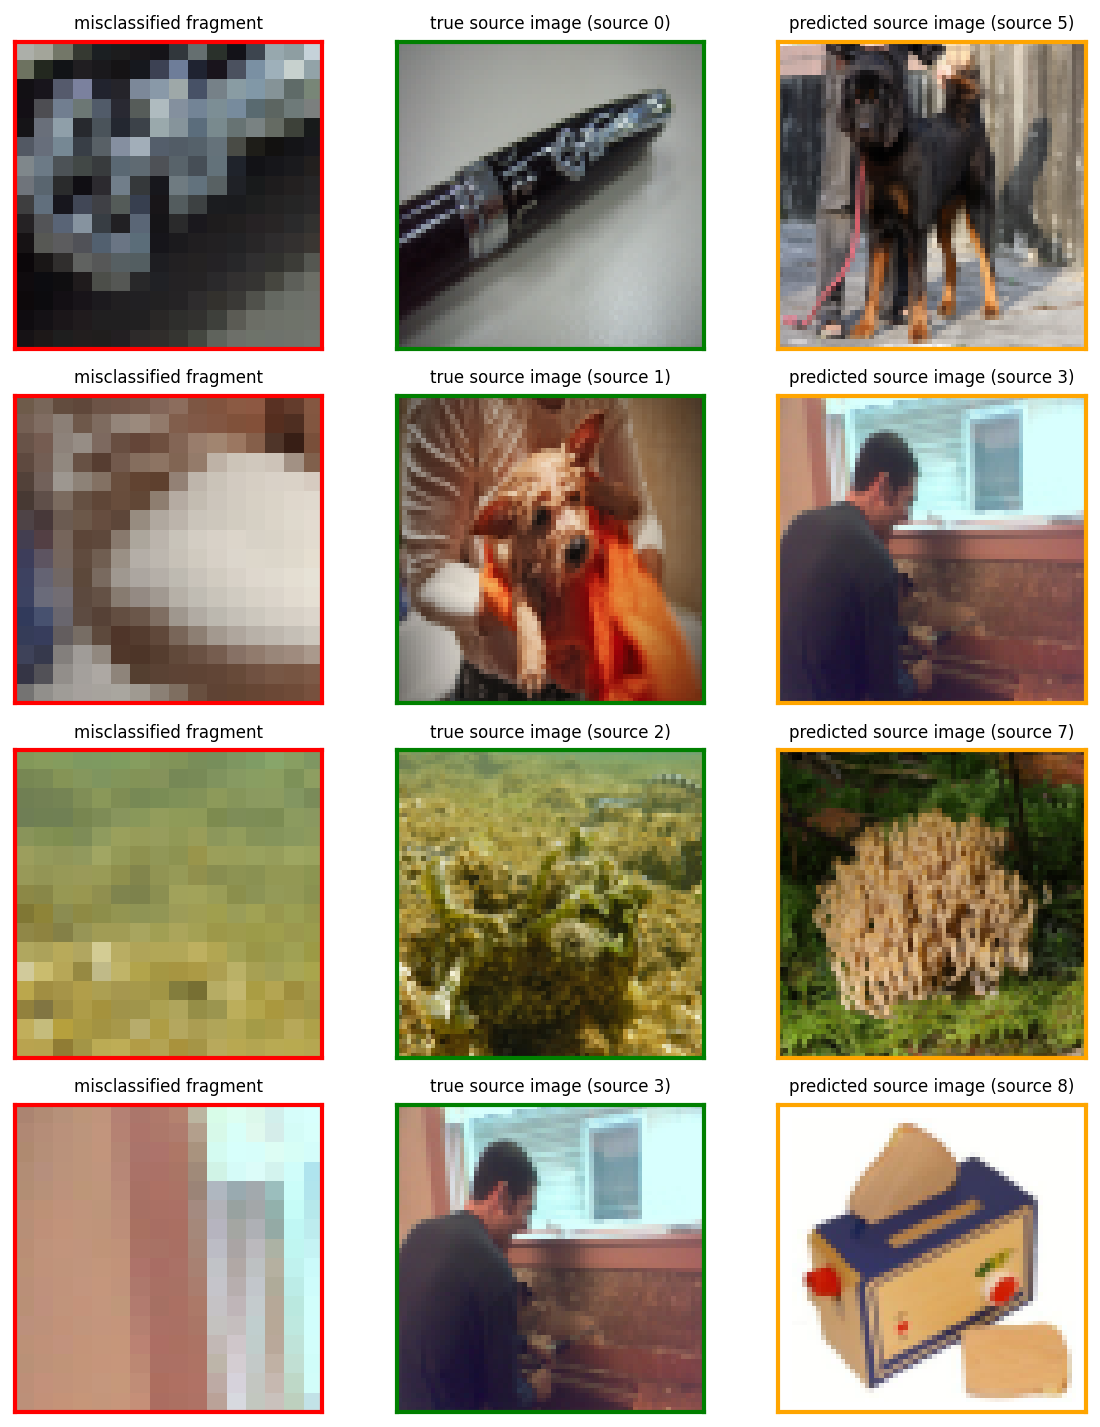
\includegraphics[width=0.85\textwidth]{failure_modes.png}
\caption{Failure modes from the current best checkpoint (\texttt{multitask_10}, best ARI = 0.570, $\beta = 0.01923$, $\lambda_{\mathrm{adj}} = 1.0$, $\lambda_{\mathrm{same}} = 1.0$, plain BCE on both heads). On the validation batch shown, 51 of 160 fragments were assigned to the wrong cluster after Hungarian matching of predicted to true labels. Each row shows: the misclassified fragment (left, red), the true source image it came from (middle, green), and the source image the model assigned it to (right, orange). Failures are dominated by near-uniform low-information fragments where multiple source images share the same dominant colour or texture --- an intrinsic ambiguity that no model trained on these $16 \times 16$ patches can resolve.}
\label{fig:failure-modes}
\end{figure}
